\documentclass[010-intro.tex]{subfiles}

\begin{document}

Personas come from the field of product design
where they are used by designers to help create products for their users.
Personas initial conception was created around people succumbing to technology that
function, but are clunky to work with
(e.g., video cassette records, car alarms, computer software applications).
The goal of a persona is to provide a user-centered approach to product design
by clearly defining remember-able representations of users.
This means trying to identify who the users are,
what they want from the product, and
how they will use the product.
The specifics and understanding that personas are representations of target groups
is what separates it from devolving into a stereotype
\cite{pruittPersonaLifecycleKeeping2006}.

Persona methodology can be applied to education as well.
The ``product'' is typically a lesson plan or curriculum,
and the ``users'' can be teachers
\cite{zagallo2019through}
or students.
This dissertation explores the use and creation of personas for learning materials
(Section \ref{sse:intro-learner-personas}).
The notion between a persona and a stereotype is somewhat related,
i.e., we hypothesize that many domain experts (e.g., medical practitioner)
do not work with data regularly,
lack data literacy concepts,
and mainly interface with data in Excel.
What sets this work apart is this hypothesis is tested and incorporated into specific
personas that have actionable decisions when putting together learning content.

\subsection{Personas}

We will begin with the basics and overview of persona methodology
before applying it to educational contexts

    \subsubsection{User-Centered Design (UCD)}

        There are three (3) main difficulties with user-centered design (UCD).
        First,
        the natural tendency is to be more self-centered, not user-centered.
            Design choices typically stem from our own wants and needs,
            and we even seek out users who are similar to ourselves for product feedback
            \cite{pruittPersonaLifecycleKeeping2006, tognazziniTogSoftwareDesign1748}.
            Self-centered design is a better approach than technology-centered design,
            where the focus is around capabilities of the technology and less around capabilities of the user,
            but most people who develop the product are not representative of the audience
            \cite{pruittPersonaLifecycleKeeping2006}.

        Second,
        Users are varied, and it is not possible to please everyone.
        Attempt to do so usually have conflicting solutions and are not possible to satisfy everyone's needs
        \cite{pruittPersonaLifecycleKeeping2006}.

        Lastly,
        the people who collect user and market research are typically not the same people as the ones who
        design and build a product.
        If the user and market data are not available at the appropriate time,
        the people who implement the product will follow a path of what is easiest and cheapest to build
        \cite{pruittPersonaLifecycleKeeping2006}.

    \subsubsection{``Users'' are Ambiguous}

        ``Users'' are an ambiguous, ill-defined, catch-all term.
        It is more or less meaningless.
        More details are needed about the ``user'' to build effective products.
        What once was a novel approach to product design is now ineffective and ambiguous as it was overused in discourse.
        We do not refer to cars, bicycles, and chairs as
        ``driver-friendly'',
        ``cyclist-friendly'', or
        ``bum-friendly'', respectively,
        \cite{pruittPersonaLifecycleKeeping2006}.
        So, we should not have to describe teaching and learning materials as ``learner-friendly''.

        Understanding and identifying users are necessary but insufficient for good design.
        There are multiple steps beyond identifying users:
        (1) user information needs to be communicated to product designers,
        (2) product designers need to interpret the information the same way,
        (3) information about the users need to be incorporated into the product, and
        (4) the design needs to be evaluated for effectiveness
        \cite{pruittPersonaLifecycleKeeping2006}.

    \subsubsection{User Representations}

        Several important milestones on user representations led to what eventually became known as ``personas''
        \cite{pruittPersonaLifecycleKeeping2006}.
        The ``market'' of people needed to be clearly identified, created, and specified and
        successful products come from specific definitions of target customers
        \cite{sissorsWhatMarket1966, winstonDefiningYourMarket1998, pruittPersonaLifecycleKeeping2006}.
        However, market-segment definitions are usually impersonal and abstract, and focusing on
        customers using ``target customer characterizations'' deeply explore individual customers in their work environment
        \cite{mooreCrossingChasmMarketing1991, pruittPersonaLifecycleKeeping2006}.
        Each characterization incorporates:

        \begin{enumerate}
            \item Personal profile and job description
            \item Technical resources
            \item A ``day in the life'' dramatization before the introduction of the proposed product
            \item Problem or dilemma that motivates the purchase of the proposed product
            \item A ``day in the life'' after the introduction of the product
                \cite{mooreCrossingChasmMarketing1991, pruittPersonaLifecycleKeeping2006}.
        \end{enumerate}

        Instead of looking at target audiences as a part of a mass population,
        the notion of ``indivisualization'' places an emphasis of looking at target audiences as individuals
        \cite{upshawBuildingBrandIdentity1995, pruittPersonaLifecycleKeeping2006}.
        Descriptive profiles describe the audience from the point of view of others,
        while individualized profiles contextualize individuals during a purchase decision as they see themselves
        \cite{upshawBuildingBrandIdentity1995, pruittPersonaLifecycleKeeping2006}.

        The need for a clearer customer ``image'' begins to bridge the gap between marketing and product design
        \cite{melloCustomercentricProductDefinition2003, pruittPersonaLifecycleKeeping2006}.
        These images use data to create single sentences that describe some essential characteristic of the customer;
        desires and suggestions for solutions are not a part of the image statement.

        Scenarios are used to aid in product design.
        These are stories about the target population,
        not specific users,
        that provides an overview of everything that is happening to help designers and analysis focus on people and tasks
        \cite{carrollScenarioBasedDesignEnvisioning1995, pruittPersonaLifecycleKeeping2006}.
        One of the major limitations with scenario-based designs is how it makes many assumptions
        about the user to describe the network of interactions,
        therefore lacking many user-level details in the environment,
        e.g., relevant details, motivation, preferences, etc.
        However, scenarios still complement persona methods to promote good UCD
        \cite{mikkelsonIncorporatingUserArchetypes2000, pruittPersonaLifecycleKeeping2006}.

        User profiles are detailed representations of users that come from data.
        These profiles are highly specific, to the point of lacking personality,
        and provide value to the product design process by consolidating
        user data from interviews and qualitative research methods
        \cite{redishUserTaskAnalysis1998}.
        User roles, on the other hand,
        provide
        (1) larger context of the user in the environment,
        (2) user characteristics within the role, and
        (3) special criteria to support the role.
        User roles are a precursor to personas and should be explored before personas are created
        by mapping roles, relationships, and tools together using ``contextual design''
        \cite{constantinePersonas2001, holtzblattContextualDesignDefining1997, holtzblattPersonasContextualDesign2002, tahirWhoOtherSide1997}.

        User archetypes are also a data-driven method created to improve on the concept of user classes and contain user
        descriptions; attributes; computer skills; concerns and goals; market size and influence; and activities
        \cite{mikkelsonIncorporatingUserArchetypes2000}.
        Personas are imaginary people used to represent a group of users.
        They are ``hypothetical archetypes'' that are created with rigor and precision, which provide its usefulness.
        Personas can be created initially as ``assumption personas'', and backed by data during the persona lifecycle.
        Using personas in Goal-Directed Design\texttrademark are used to inform product design for lasting solutions
        \cite{cooperInmatesAreRunning1999, pruittPersonaLifecycleKeeping2006}.

    \subsubsection{Using Personas}

        There are four (4) main benefits to using personas:

        \begin{enumerate}
            \item Make assumptions about users explicit
            \item Place the focus on specific types of users rather than on all possible users
            \item Help us make better decisions by limiting choices
            \item Engage the product design and development team
                (\cite{pruittPersonaLifecycleKeeping2006, schwartzParadoxChoiceWhy2016})
        \end{enumerate}

        Just creating the personas is not enough.
        They need to be used in a thoughtful way.
        Collecting and analyzing user data is the start of creating a report about the users.
        But these reports also need to be created with the people who implement the product in mind.
        Many times, a partial understanding of the indented product user gets
        tinted with personal experiences and biases,
        and the user report, along with its original message, largely gets underutilized
        \cite{pruittPersonaLifecycleKeeping2006}.

        It's impossible to cater to every persona,
        nor should all possible types of users be made into a persona.
        The notion of a primary persona is crucial for managing effort and resources.
        Even if the personas created were ``wrong'',
        the personas were created from user data and the ``finished'' persona is only the starting point
        that needs to be validated with more user research.
        At worst, using a ``wrong'' persona still provides a consistent product
        \cite{pruittPersonaLifecycleKeeping2006}..

        This dissertation seeks to identify medical practitioners as its main persona,
        and use a series of targeted survey questions to distinguish key components
        of data literacy topics and technical programming skills, they are lacking.
        The learning materials created will primarily depend on their relevant prior knowledge,
        and their perception of needs.

\subsection{Learner Personas in Education}
\label{sse:intro-learner-personas}

    The primary user role for this dissertation are people who work in the biomedical sciences
    (e.g., students, researchers, and medical clinicians)
    who are data science novices.
    This body of work seeks to collect user data (i.e., learners) to create personas (i.e., learner personas)
    to better engage learners and aim to improve learning outcomes (Table \ref{tab:persona-comparison}).

    \begin{table}[!hbtp]
        \centering
        \caption[Personas vs Learner Personas]{
            How learners can be the ``user'' in product (i.e., lesson) design.
            The personas column are reproduced from ``The Persona Lifecycle'' \cite{pruittPersonaLifecycleKeeping2006}
            were corresponding list for learner personas were adapted from.
        }
        \begin{tabular}{p{0.45\linewidth} | p{0.45\linewidth}}
            \hline
            Personas                                                                                         & Learner Personas                                                                           \\
            \hline
            \textbullet Increase your products' usability, utility, and general appeal                                & \textbullet Increase a lessons' usability, utility, and general appeal                                 \\
            \textbullet Streamline your teams' processes and improve your colleagues' ability to work together        & \textbullet Streamline learning progress and improve learner team Interoperability     \\
            \textbullet Enable your company to make business decisions that help both your company and your customers & \textbullet Enable learners to make data-driven decisions  \\
            \textbullet Improve your company's bottom line                                                            & \textbullet Improve learning outcomes \\
            \hline
            \end{tabular}
        \label{tab:persona-comparison}
    \end{table}

    Creating learner personas is not a new concept in education.
    They have been created for teachers to identify what kind of professional development needs they have
    (Figure \ref{fig:teaching-personas}) \cite{zagallo2019through},
    and in industry to identify the kinds of learning resources and documentation
    are needed to better use their products
    (Figure \ref{fig:rstudio-learner-personas}) \cite{rstudioLearnerPersonas2019}.
    The personas created by The Carpentries \cite{softwarecarpentryLearnerProfiles} and RStudio, PBC \cite{rstudioLearnerPersonas2019},
    include ones that are looking for data science training.
    What is lacking are explicit personas for specific domains.
    This can help identify common knowledge bases to better curate learning materials
    (Section \ref{se:intro-teaching-best-practices-ds}),
    and also serve as marketing and outreach materials to help learners find resources
    \cite{wilson2019teaching}.

    \begin{figure}[!hbtp]
        \centering
        \includegraphics[width=\textwidth]{050-intro/rstudio-learner\_persona.PNG}
        \caption[RStudio Learner Personas]{
        Learner personas}
        \label{fig:rstudio-learner-personas}
    \end{figure}

    \begin{figure}[!hbtp]
        \centering
        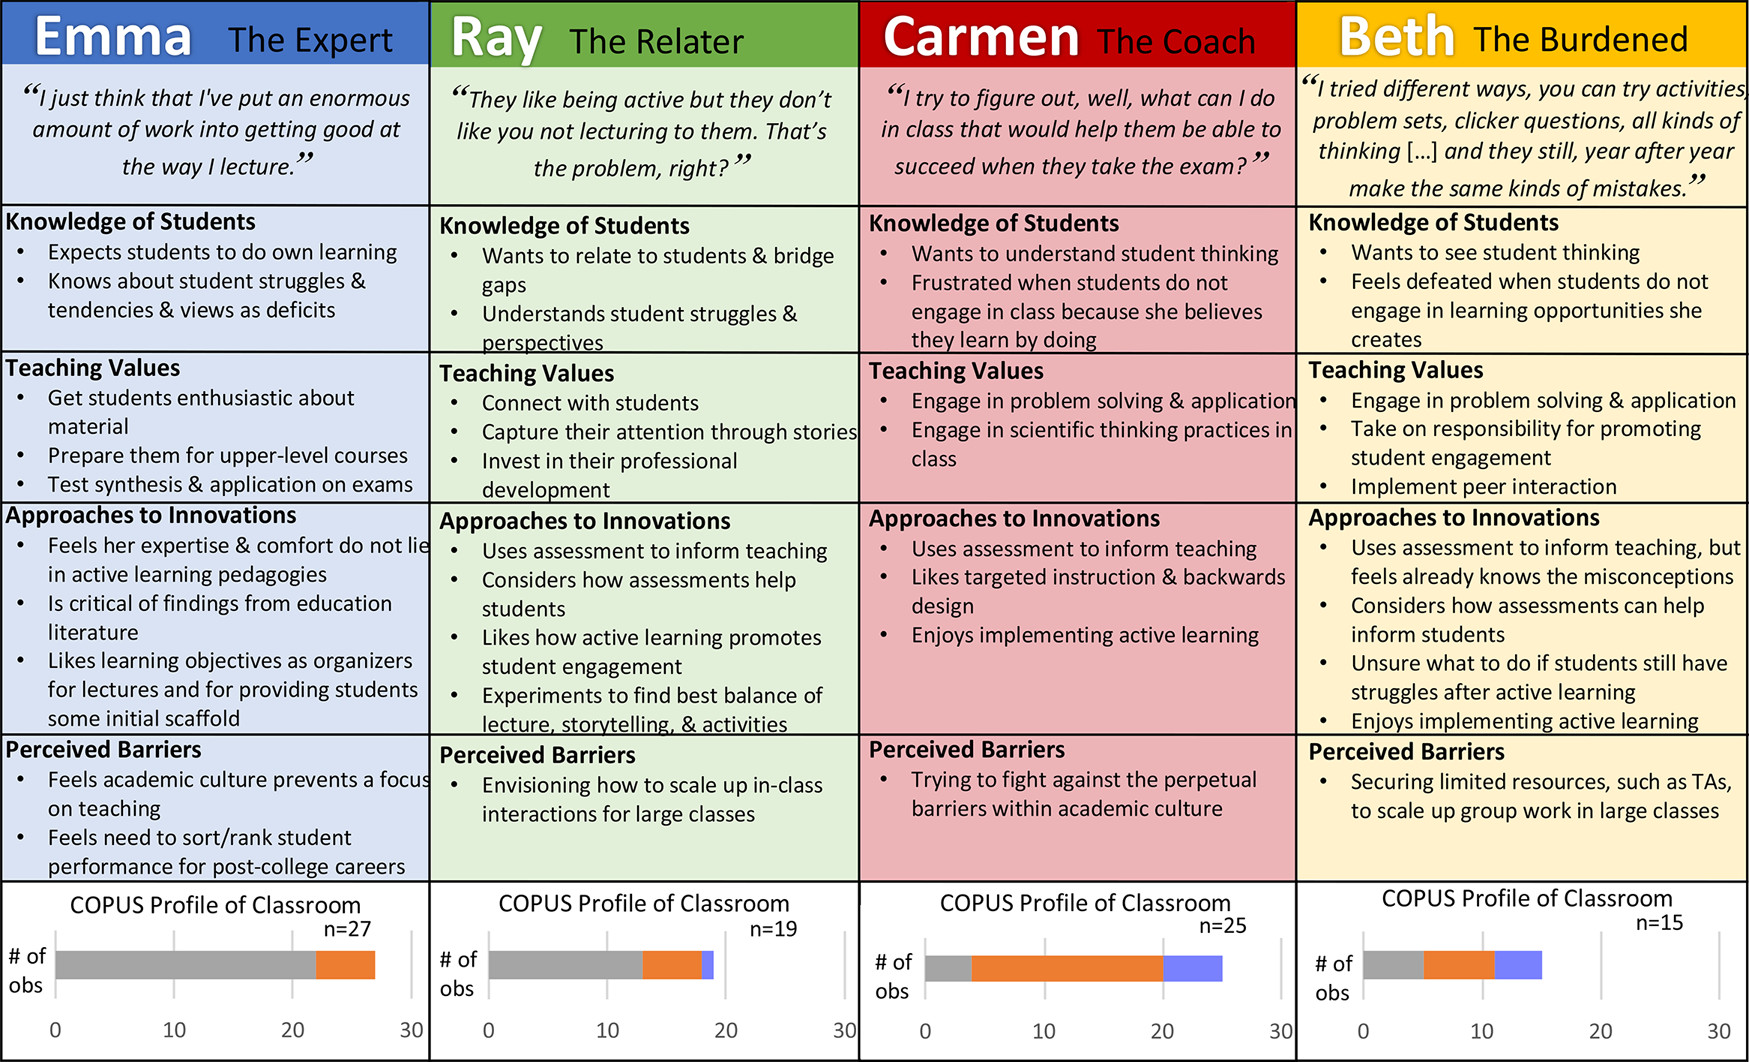
\includegraphics[width=\textwidth]{050-intro/zagallo-2019--fig_2.jpeg}
        \caption[Reproduced Teaching Personas \cite{zagallo2019through}]{
        Reproduced Teaching personas \cite{zagallo2019through}.
        These show the 4 personas created looking at professional development needs for teachers.
        }
        \label{fig:teaching-personas}
    \end{figure}



\end{document}
